\begin{columns}
\begin{column}{.25\textwidth}
\justify
The following instruction table is a simplified example of description of a pseudo-vector instruction set. The actual table for production use would contain intrinsic functions in patterns. We reckognize the following constructs: operation, instruction, type, type version, width conversion, expansion, although flat format flattens some of these constructs into a single line. The second figure shows non-flattened hierarchy of the structures.
\end{column}

\begin{column}{.02\textwidth}
\end{column}
\begin{column}{.38\textwidth}
\begin{verbatim}
#type       type in out pattern                       pattern2
conversion  INT  2  1   $arg1 (b & 0xFFFF0000) >> 16  $arg1 & 0xFFFF
conversion  INT  1  2   $arg1 | ($arg2 << 16)

#type       id   width  pattern
type        INT  1      uint16_t
type        INT  2      uint32_t

#type       id   intpe  outtpe in out pattern
instruction MOD4 INT    INT    1  1   $arg1 % 4
instruction MOD4 INT    INT    2  2   $arg1 & 0x00030003
instruction LD          INT    1  1   $input
instruction ST   INT           1  1   $output
\end{verbatim}
\end{column}

  \begin{column}{.3\textwidth}
  
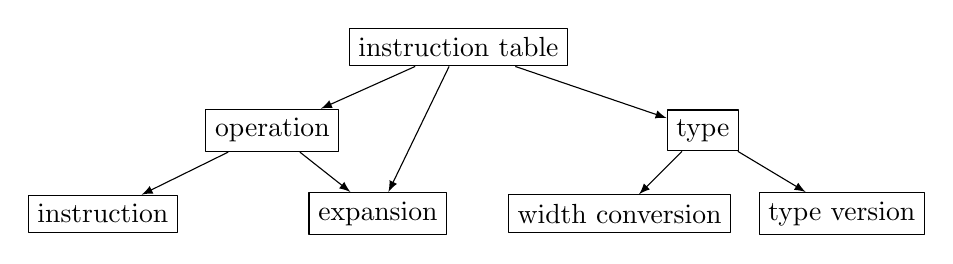
\begin{tikzpicture}[>=latex,line join=bevel,]
%%
\node (conv) at (225bp,10bp) [draw,rectangle] {width conversion};
  \node (tv) at (305bp,10bp) [draw,rectangle] {type version};
  \node (ins) at (39bp,10bp) [draw,rectangle] {instruction};
  \node (exp) at (138bp,10bp) [draw,rectangle] {expansion};
  \node (instab) at (167bp,70bp) [draw,rectangle] {instruction table};
  \node (type) at (255bp,40bp) [draw,rectangle] {type};
  \node (op) at (100bp,40bp) [draw,rectangle] {operation};
  \draw [->] (instab) -- (op);
  \draw [->] (instab) -- (type);
  \draw [->] (instab) -- (exp);
  \draw [->] (op) -- (ins);
  \draw [->] (type) -- (tv);
  \draw [->] (op) -- (exp);
  \draw [->] (type) -- (conv);
%
\end{tikzpicture}


\end{column}

\end{columns}

